%
%  Thesis 
%
%  Created by Johan Grahn on 2009-01-28.
%  Copyright (c) 2009 Högskolan i Skövde. All rights reserved.
%
\documentclass[MSc, ida]{histhesis}

% Setup for fullpage use
%\usepackage{fullpage}

% Uncomment some of the following if you use the features
%
% Running Headers and footers
\usepackage{fancyhdr}

% Be able to rotate tables
\usepackage{rotating}

% Multipart figures
%\usepackage{subfigure}

% More symbols
%\usepackage{amsmath}
%\usepackage{amssymb}
%\usepackage{latexsym}

% Surround parts of graphics with box
\usepackage{boxedminipage}

% Package for including code in the document
\usepackage{listings}

% This is now the recommended way for checking for PDFLaTeX:
\usepackage{ifpdf}

\usepackage{graphicx}

% Set equal margins on book style
%\setlength{\oddsidemargin}{53pt}
%\setlength{\evensidemargin}{53pt}
%\setlength{\marginparwidth}{57pt}
%\setlength{\footskip}{30pt}

\usepackage[utf8]{inputenc}
\usepackage{natbib}

\setcounter{tocdepth}{2}

\title{EPRiDe}
\subtitle{A performance evaluation}
\author{Johan Grahn}
%\course{Magisterexamen, Avancerad nivå, 30 hp}
\supervisor{Gunnar Mathiason}
\semester{Spring 2009}

\begin{document}
\maketitle
\begin{abstract}

(<<<< Write an abtract >>>>)

\end{abstract}
\tableofcontents
\thispagestyle{plain}
\listoffigures
\newpage
%!TEX root = /Users/high/Documents/School/Thesis/report/thesis.tex
\section{Introduction}
\label{sec:intro}

When using distributed databases, replication is an important factor for increasing reliability and availability. A distributed database system needs to be fault tolerant so that if any database node is unavailable, the application selects a new one without need for client interaction. 

In replication, there exists different replication approaches. Two of them are pessimistic and optimistic replication. Pessimistic is most commonly used and guarantees mutual consistency in distributed database systems, but are to restrictive for most real-time database systems. Optimistic replication increases availability at the cost of consistency. 

In a distributed real-time databases(DRTDBMS), there is a need for resource predictability. Transactions need to have predictable execution time or deadlines can be missed which can cause catastrophic consequences, e.g. losing lives.
\newpage
%!TEX root = /Users/high/Documents/School/Thesis/report/thesis.tex

\section{Background} % (fold)
\label{sec:background}

\subsection{Transactions in Database systems}
\label{sub:db}

A transaction, as defined by \cite{Elmasri2004}, is an atomic unit of work that is either completed in its entirety or not at all. A transaction contains a number of operations that can either write to the database or read from the database. 

When a database uses transactions, there are a number of states that the database needs to record about each transaction \cite[]{Elmasri2004}:

\begin{description}
	\item[Begin] This means that a transaction have been started
	\item[Read or Write] A read or write operation that is performed inside the transaction
	\item[End] Marks the end of the transaction when all read and write operations have been performed that is defined inside the transaction
	\item[Commit] This stores the operations permanently into the database 
	\item[Rollback or Abort] This state says that the transaction should be aborted and all operations inside the transaction need to be undone.
\end{description}

% The database store a log with all operations that have been performed inside the transaction, so the database can undo all operations if a rollback is performed or if a commit is performed, the database knows what operations that are permanently stored in the database. 

Transactions should have the ACID properties \cite[]{Haerder83}, so that each transaction doesn't affect another transactions validity. These properties are defined as:

\begin{description}
	\item[Atomicity] This means that all operations that are defined in the transaction are performed, or none of the operations are performed.
	\item[Consistency] This means that the database should be in a consistent state after the transaction has performed the operations. No violations, for example in table constrains, can occur. 
	\item[Isolation] The transaction are not interfered by any  other transaction that are executing concurrently. This is to prevent any concurrency problems.
	\item[Durability] This means that when the transaction is committed, the changes that where made in the database needs to be stored permanently, and the changes can't be lost. 
\end{description}


\subsection{Distributed Database Systems} % (fold)
\label{sec:distributed_database_systems}

A definition, given by \cite{prins99}, is that a distributed database system(DDBMS) is a collection of multiple logically interrelated databases distributed over a network. DDBMS has number of advantages over central database systems. This includes data independence, network transparency and replication transparency. Data independence means that the physical location of data is not known to the user application. Network transparency means that network details are not known to the user application and sees the database as local. Replication transparency means that data is replicated without user interaction for performance, reliability and availability.

In a DDBMS, when a transaction needs to update more then one node in the network, a distributed transaction is used. Distributed transactions are a definition of nested or flat transactions \cite[]{Coulouris2005dsc}. Flat transactions means that updates are performed on a number of nodes that are linked to the coordinator of the transaction. Nested transactions are when updates on a number of nodes that are linked to the coordinator, creates updates that need to be performed on another number of nodes in the network building a tree-like structure. 

\subsection{Replication} 
\label{ssub:replication}

In distributed databases, replication is used to increase availability and fault-tolerance of the system. In this report, a replica is a copy of a object located on the same node or on another node. A client is an application that uses some or all data that is stored inside the database. 

There exists a number of different type of replication styles. Most commonly used are \emph{pessimistic replication} and \emph{optimistic replication}. Pessimistic replication is most commonly used in database systems and the idea is to maintain single-copy consistency, which means that every replica are consistent with each other and a client will always the updated data. This type of replication is to restrictive since a client are not allowed to read from a replica unless that replica is updated with the latest data. 

Optimistic replication uses a more ``optimistic'' approach. The idea is to allow replicas to diverse at first, and resolve any conflicts that have occurred later. In optimistic replication, the update is committed locally first, and then updated are propagated to the other replicas, integrate the update in the replica and lastly performs conflict resolution \cite[]{saito2005}. This increases the availability of each replica and the protocol can handle network partitioning.

When using optimistic replication, there are a number of different configurations in how many \emph{replica writers} that system has \cite[]{saito2005}. \emph{Single-master} is when only on replica writer is allowed. All updates are send to the same master that updates locally and then replicates to all other replicas.  This type of architecture is simple, but has low fault-tolerance since all requests need to be processed and replicated by the master which means that the master is a single point-of-failure. \emph{Multi-master} is when the systems allows more than one replica writer. In multi-master, all updates are performed locally on each replica and are then send to the other replicas in the background. This allows better scalability and availability, but at the cost of consistency. Multi-master guarantees only eventual consistency, which means that the client must tolerate that the data that the client reads can be changed due to a conflict resolution.   	   


\subsection{Database Consistency} % (fold)
\label{sub:consistency}

For replication, different consistency guarantees can be given depending on what type of replication that is being used. In pessimistic replication, mutual consistency is guaranteed. This is used when applications doesn't tolerate any inconsistent data between replicas. Optimistic replication only guarantees eventual consistency, which means that the replicas will eventually be consistent if there no new updates are send to any replica. One problem with eventual consistency is that an application need to tolerate occasional conflicts \cite[]{saito2005}. This mean that the application needs to tolerate that it sometimes reads unstable data and that a value can be updated in the future until it is stable. A stable value is a value that is permanently stored in the database and will be consistent on all replicas.


\subsection{Distributed Real-time Database Systems} % (fold)
\label{sub:subsection_name}

In a distributed real-time databases(DRTDBMS), there is a need for resource predictability. Transactions need to have predictable execution time or deadlines can be missed which can cause catastrophic consequences, e.g. losing lives. When performing distributed transactions, there is a need to know how long execution time each transaction has. With a distributed real-time database, it is hard to calculate WECT since the network is unpredictable. Network partitioning and packet losses can have huge affect distributed transactions. One solution to this that is suggested by \cite{deeds}, is to remove the unpredictability of distributed transactions by allowing replicas to diverse in data and only guarantee local predictability.  

\subsection{Conflict resolution} % (fold)
\label{sub:conflict_resolution}

When performing conflict resolution on conflicting updates, most systems tries to revert the system to a previous state that was considered to be safe, called \emph{backward} conflict resolution. The problem is that embedded and real-time systems some actions can be external and can't easily be undone (drilling a hole into a wall for example). This creates problems when trying to abort a transaction. 
With \emph{forward} conflict resolution, actions are performed to take the system into a new state that is considered to be safe.      

% subsection conflict_resolution (end)

\subsection{PRiDe}
\label{sub:pride}

The PRiDe protocol used in DeeDs DDBMS \cite[]{deeds}, is a optimistic replication protocol with support for forward conflict resolution \cite[]{Syber2007}. 

PRiDe builds on the Continuous Convergence(CC) protocol \cite[]{consistency2005}, which is designed to meet three database requirements: 
\begin{description}
	\item[Local consistency] means that the transactions should generate a consistent state on the local node
	\item[Local predictability] Means that the transaction should have predictable resource usage and execution time to meet the requirements of realtime-systems.  
	\item[Eventual global consistency] means that the database should eventually be consistent, if there is no new updates that are send to the database nodes.  
\end{description}    

In PRiDe, eventual global consistency is achieved by the fact that  updates are continuously propagated to all replicas in the network and integrated at the replica . All updates are continuously and optimistically resolved, meaning that conflicts are resolved when they are discovered during the stabilization phase. 

\newpage
%!TEX root = /Users/high/Documents/School/Thesis/report/thesis.tex

\section{Problem description}
\label{sec:problem_description}

%In a distributed database system that uses single-master replication, receive all updates to a specified database node, called master node, performs the updates locally, and then replicate data to the other database nodes in the network. There are two problems with this approach, predictability and blocking time. 

%When a database node sends data to the master database node, the master node can disconnect due to network partitioning or hardware failure. Then the database node needs to wait until the master database node returns or a new master is selected. The time that the database node must wait can't  and then it is not suitable for realtime requirements.

%When a database node is performing a distributed transaction, all other update transactions is blocked until the distributed transaction has committed or aborted. Since the blocking time isn't bounded, then local predictability can't be guaranteed.  
The PRiDe protocol have currently been evaluated in two ways: In a VAD(Visual Aid Designer)er tool \cite{Syber2007} and in a protocol extension, called pPRiDe \cite[]{Olby07}. 

No full performance evaluation has been conducted, in terms of resource usage and execution. The resource usage is vital for protocols like PRiDe since the idea is that PRiDe should be used in real-time systems where the resource usage needs to be predictable and the execution time needs to be bounded. 

\subsection{Aim}
\label{subsec:aim}

The aim with this final year project is to investigate how well PRiDe performs in a real system, based on a number of defined performance metrics.  

\subsection{Motivation}
\label{subsec:motive}

Since the PRiDe protocol has only been evaluated in a simulation, there is a need for an investigation of performance and resource usage in a realistic situation \cite[]{Syber2007}.

\subsection{Objectives} % (fold)
\label{subsec:objectives}

To be able to fulfill our aim, the following objectives needs to be meet:  

\begin{description}

	\item[Define implementation scope for PRiDe] \

	There are a number of features of the PRiDe protocol that take to long to implement for the given time frame for this research project. A analysis should be performed to see what features that are needed in an implementation for performance experiments, in the time frame for the project.

	\item[Implement PRiDe on a platform] \

	For an implementation of PRiDe, a well-known distributed database platform should be used such that functionality for support database operations are already implemented and can be reused. The term platform in this project is defined as a software component that supports as much functionality as possible for an implementation of the PRiDe protocol. 

	\item[Create baseline for evaluation] \

	A baseline needs to be defined to be able to create and compare experiments to evaluate the performance. Both the PRiDe protocol have a number of requirements that the baseline needs to fulfill. For PRiDe, one requirement should be eventual consistency. For DeeDS, a requirement should be in-memory storage. An analysis needs to be conducted to see what these requirements are and to select a good candidate that fulfill the given requirements so that a correct evaluation can be performed.


	%The platform needs to be extended with distributed-master support. For an evaluation of PRiDe, support for independent updates is required. and for distributed transactions that allows updates of master data replicas from slave database nodes.

	\item[Evaluate the performance] \

	When evaluating the performance a number of performance metrics needs to be specified to be able to define the use for each experiment. A number of experiments should be defined to be able to measure each metric, such that measurements can be made to compare performance.  
	
	In this project, we need to define a number of performance metrics that we believe that can be used in the performance evaluation. These metrics are execution time, blocking time, bandwidth usage, stabilization time. Execution time is the total time it takes to replicate and stabilize each update. Blocking time is how long a transaction must wait from the time when the transaction commits until the transaction is completed. Bandwidth usage is how much messages each node in the network uses for replication and stabilization. Stabilization time is the time from that an update has been considered unstable to the time when it is stable by performing stabilization. These performance metrics are not complete and can be changed as the project progresses.
 
The evaluation should conduct measurements with three types of setups. \emph{Single-master evaluation} should evaluate the performance when only one replica writer is allowed. The idea of the test is to create a base case. \emph{Multi-master evaluation} should evaluate the performance when multiple replica writers are allowed. The idea is to see that PRiDe has lower blocking time then the defined baseline. \emph{Stabilization evaluation} should evaluate the resource usage when performing stabilization. The test should show that there is no overuse of resources.  

\end{description}
% (end)
\newpage
%!TEX root = /Users/high/Documents/School/Thesis/report/thesis.tex

\section{Method} % (fold)
\label{sec:method}

In this chapter, methods for achieving all the objectives are discussed in more detail.

\subsection{Define implementation scope for PRiDe} 
\label{subsec:impl_bound}

A literature analysis of alternative protocol specifications is conducted to achieve domain knowledge and protocol attributes about PRiDe. The protocol specification will include features that are used by PRiDe, both required and optional features to guarantee replication correctness. 

\subsection{Implement PRiDe on a given platform} 
\label{subsec:create_implementation}

Two alternatives have been identified for an implementation that follows the DeeDS architecture.

\begin{description}
 
\item[Create a layer on top of Berkley DB] \
	
A implementation of PRiDe will be implemented on top of Berkley DB, using Berkley DB as local database with replication disabled in Berkley DB. This type of implementation has also been performed in Dynamo, as described by \cite{Dynamo2007}. In Dynamo, BerkleyDB acts as local database manager with no replication support and the replication is done by a upper layer. Dynamo supports optimistic replication so that writes can always be performed(e.g. not blocked by other writes) and it supports eventual consistency so that any inconsistencies created by the replication can be resolved later. This means that Dynamo has similar features as PRiDe and motivates why PRiDe can be implemented in the same way.  
	
\item[Integrate in Berkley DB] \

The implementation will be inserted inside Berkley DB to change the replication semantics of Berkley DB and to reuse some of the features that Berkley DB has. A technical report, written by \cite{kang2008}, describes that there is a number of inter-dependencies, both in the replication layer, and between the upper replication layer and lower BDB layer. These inter-dependencies are not documented at all, and will extend the development time a lot by testing and verifying the implementation since the behavior of the replication can't be derived from the documentation.
    	
%PRiDe will be implemented as a layer above the replication layer in Berkley DB. The protocol will interpret transactions coming from  Berkley DB, and perform protocol specific instructions and then send it to the replication layer in BerkleyDB. \cite{kang2008} argues that since Berkley DB was designed for single-master replication, there are a number of inter-depedencies that make it hard to modify the replication layer.
\end{description} 

%\subsection{Extend platform for evaluation} % (fold)
%\label{sub:extend_framework}

%\subsubsection{Requirements on the platform} % (fold)
%\label{ssub:demands_on_a_framework}

%The framework should have the same features as PRiDe has (or as close as possible). This means that the framework should have support for eventual consistency, multi-master replication, and transactions. These are features that are central to the PRiDe protocol.

%The framework should also be extendable since if there are some features that are missing, there should be easy to implement on the framework. 


%\subsubsection{Review and selection of platforms} % (fold)
%\label{ssub:rev_of_framework}

%There exists a number of frameworks that are suitable for this type of extension based on their features:

%\begin{description}
%	\item[Berkley DB] 
%		Berkley DB is open-source distributed database, which matches the requirement about extendability, since the source-code can be modified. Berkley DB supports single-master replication, which is close to what we want to have, that is multi-master replication.  Berkley DB also supports transactions which also are needed for the experiment. 
	
%	\item[Polyhedra] 
%		Polyhedra is a distributed database. It supports transactions, in-memory data storage and single-master replication.  Polyhedra is based on a client/server architecture with cross-platform interpretability. 
%	\item[Mimer SQL Real-Time Edition]
%		Mimer DB is a distributed database with support for transactions, single-master replication and real-time constraints.
%\end{description}

%Table \ref{table_features} gives a summary of support for the features that are needed by DeeDS.

%\begin{table}[h]
%	\begin{tabular}{r|c|c|c|c}
%		& \textbf{Extendable} & \textbf{Ev. Con.} & \textbf{Multi-master} & \textbf{Transactions} \\ \hline
%		BDB & X & - & - & X \\
%		MimerDB & - & - & - & X \\
%		Polyhedra & - & - & - & X \\ 
%	\end{tabular}
%	\caption[Database features]{Table showing what features the databases support that are required by DeeDS}
%	\label{table_features}
%\end{table}

%Given the features that each framework has, the chosen framework for this study is Berkley DB. Both Polyhedra and Mimer SQL supports both transactions and single-master replication as BerkleyDB but in both cases, there is a need for a license. Berkley DB is open-source, which means that there is no need for a license and can be modified in any way that is necessary. Since Polyhedra is based on a client/server architecture it would take longer time to extend then Berkley DB because Berkley DB is just a static library that you include in your source code which removes the time for developing the client for using the Polyhedra client library.  

\subsection{Evaluate the implementation} 
\label{subsec:experiment}

\subsubsection{Evaluation definitions} % (fold)
\label{ssub:evaluation_baseline}

For the experiments, we define a baseline that we can evaluate with. This baseline consists of two systems. The first system is general distributed database(DDB) that uses single-master replication and uses a two-phase commit protocol. DDB will only be used as a baseline for discussing, and will not be used in the experiments. The second system is Berkley DB but has been extended with multi-master support, will be referenced as BDBe (Berkley DB extended). 


% subsubsection experiment_systems (end)
\subsubsection{Performance metrics} % (fold)
\label{ssub:performance_metrics_discussion}

When measuring performance, a number of performance metrics should be established. The metrics that are defined below have been chosen because these can (in some degree) be measured in each of the systems that are going to be used in the evaluation.
%To be able to perform a number of performance measurements, there are different performance characteristics that need to be addressed. In this report a number of metric will be used based on the fact that these can be measured equal in  single-master, the used framework and in PRiDe. 

\begin{description}
	
	\item[Bandwidth usage]

This metric is measured can be measured in two ways. Measuring the amount of data traffic that gets transfered between two database nodes in the network or measuring the total number of data that is transfered between all the replicas in the network during the entire experiment.

	\item[Execution time]
	
	This metric measures the time it takes to process all transactions and to the time when all replicas has the same information about all objects that have been updated. For PRiDe, this means that the time for receive all transactions, perform local integration, propagate to all the replicas, perform integration on the target replica, and finally perform stabilization on target replica. For DDB, it is the time for receiving all transactions, and performing a distributed transaction update each replica. For BDBe, it is to process all transactions and for each transaction, perform local integration on the master node, and then replicate the update to the slave replicas and perform integration on the each slave. When only one node receives the updates. If all nodes can receive updates, execution time for BDBe is the time to receive all transactions, send all transactions to the master node, propagate the updates to the replicas and then integrate the update on the target replica.
	 
	%This is the time it takes for each database node to process each transaction and perform a commit or abort on the transaction, and then replicate the update to the other database nodes and integrate the update and the database node. 
	
	\item[Stabilization time]
	This mean the time from that a update has reached a replica and until the update is stable on that replica. This is only measurable on PRiDe because there is no stabilization in DDB, and in BDBe, the stabilization time is from the time when the local integration has performed on master nod and until the update has been propagated to the target replicas and have been integrated on target replicas. But these is not stabilization, it is just replication of an update.
	
	In PRiDe, this can be measured on individual node, by measuring the time it take from that an update has been locally integrated on the replica and to the time when the update have been moved to the stable prefix. This includes the time it takes to perform conflict resolution. 
	
	The type of measurements can be compared between different replicas. This means that measurements can done by the maximum time, minimum time, average time, when comparing with all replicas in the network. 
	    
	%This is the time it take for each database to process each transaction, commit or abort locally and then replicate the update to the remove database nodes, and integrate the update, and finally pertform stabilization on the updates so that all database replicas have the same information about all objects.
	 
	\item[Blocking time] 
	
	When only one node (master node) is allowed to perform updates, the blocking time for PRiDe is only the time it takes to make a integration of the update on the local node. For DDB, the blocking time is the time when the transaction waits until all (or some) of the replicas has integrated the update. For BDBe, this means that blocking time will just be the local blocking time for performing the commit.
	When independent updates are allowed, it is the same blocking time for PRiDe, but for BDBe, each transaction need to wait for the transaction to be send to the master node and integrate the update on the master and then receive a reply. The blocking time for BDBe can be affected by network latency and network partitioning. For DDB, independent updates can't be used since only one node (master node) can receive updates.
	
\end{description}

%\begin{figure}[th]
%\centering
%\includegraphics[scale=0.50]{PRiDe_metrics.pdf}
%\caption{Transverse momentum distributions}\label{fig:testing}
%\end{figure}

\subsubsection{The experiments} % (fold)
\label{ssub:the_experiments}

Three experiments have been identified that evaluates the defined performance metrics. The first two are required for this experiment, and the third experiment is optional based on the fact that is performs a validation, and not a comparison:

\begin{enumerate}

	\item \textbf{Single-master replication} \\ In this experiment, execution time and bandwidth usage will be measured and only one node will receive the transactions. For DDB, and BDBe this means that all transactions will be received on the master node. This is to measure ho much overhead PRiDe has when performing stabilization, since DDB and BDBe doesn't need to perform any stabilization since they guarantees mutual consistency. The hypothesis is that PRiDe will have none or a small overhead since every update creates a new generation that needs to be stabilized in a stabilization phase.
	
	\item \textbf{Multi-master replication} \\ In this experiment, transactions will be received on all nodes in the network for evaluating how BDBe and PRiDe handle independent updates. Execution time, blocking time and bandwidth usage will be measured. Since BDBe have some blocking time during each transaction, PRiDe should have higher throughput of updates that are locally integrated into the node that receives the update.  
	
%In this experiment, there is an interest to measure blocking time, since every node that is not a master, needs to wait until a transaction has been received, committed and propagated until next transaction can be processed. Bandwidth usage is also a interesting factor here, because this test should show that PRiDe uses less bandwidth since each transaction can be commit locally, so there is no need to send it to a master node. Execution time will also be measured since this is of interest to find out how long it takes to get all transactions performed on all nodes. A hypothesis here is that PRiDe should perform this experiment better since BerkleyDB needs an extra transfer to the master node on each transaction. 
	   
	\item \textbf{Stabilization resource usage} \\ In this experiment, the stabilization time will be measured. This will only conducted with PRiDe to evaluate if there are any spikes in resource usage when performing stabilization and conflict resolution. In this experiment .
	
%Last experiment the idea is mainly to measure the stabilization time. For PRiDe, this means that the time it takes to stabilize all object and resolve any conflicts. In BerkleyDB, this means measuring the time it takes to process all updates for the master and then propagate the information to the slaves. 
	 
\end{enumerate}

%Next experiment should be to see how PRiDe performs when using distributed masters in a network. Since BerkleyDB only has support for single-master, it must send each transaction to the master node so that master node can make a commit and then propagate the update to all nodes in the network and finally report back to the database node that send the transaction that it was committed or aborted.  A hypothesis here is that this should take longer to performs this task then with PRiDe because in PRiDe all database nodes are allowed to run transactions independent of each other. In the case of BerkleyDB a increase in execution time and bandwidth usage should be shown because two additional messages transactions needs to be performed.  

%A final experiment should be to test how PRiDe is performed in database network with multi-master replication. The purpose is manly to measure stabilization time but execution time and bandwidth usage should also be measured. Stabilization time can be measured in different ways. It can be measured on each individual node or measure it from start until all database nodes have propagated all updates and have integrated all updates on their local copy. Measuring on a individual node doesn't give any result that can be used since it depends on network latency when each database node receives its messages. 

\newpage
%!TEX root = /Users/high/Documents/School/Thesis/report/thesis.tex

\section{Architecture} % (fold)
\label{sec:arch}

In this section, a description of the overall architecture that are used in the implementation will be explained in more detail.  

% (end)

\subsection{Concepts} % (fold)
\label{sub:consepts}

In an application that needs replication, there is a distinction between \emph{local objects} and \emph{database objects}. Local objects are temporary objects that the application uses but there is no need to store these objects for later use. Database objects are objects that are used in the application and are durable, which means that the object can't be lost if any error occurs. These objects needs to be replicated 

A database object is associated with a unique database object identifier(DBOID) that is unique between all EPRiDe nodes in the network. This is means any logical object in a EPRiDe instance can't have the same identifier as another object on the same EPRiDe instance or on any other instance in the network.    

A database object can store primitive data types. This includes for example int, char, double. Pointer to other database objects are not handled are out of scope for this implementation since it creates more complexity in recording state of each object. One possible solution is to define a interface that has a number of operations that are handled by EPRiDe and are mapped to objects that handles the actual method that is defined in the interface.    

A database object can only read and write data. Database objects are not allowed to send messages to other database objects since these messages can create inconsistency between EPRiDe instances.

To be able to store all updates that are performed on database object, EPRiDe logs each operation that is performed on the database object. Operational logging is better to used since it increases the semantics used in conflict resolution compared to value logging, where only the result of the operation are logged. 

%To be able to store information about each operation that are performed on a object, EPRiDe logs each operation that is performed a method call object(MCO) are created. 

%Each MCO stores information about the DBOID, the operation that have been called, and the parameters that are being send to the operation. 

% (end)

\subsection{Network} % (fold)
\label{sub:network}

In a system that uses EPRiDe, each node in the network is an instance of EPRiDe. These instances communicate with each other only through message-passing. 

\subsection{Components} % (fold)
\label{sub:components}

Each EPRiDe instance consists of a number of components:

\begin{description}
	\item[Application] \
		The application component is responsible for handling read and write requests that an application can make. This includes transaction commands.
		
	\item[Propagater] \
		The propagater is responsible for sending updates that are in the conflict set to the other EPRiDe instances. The propagater is used  when a commit has been performed on the node and the information needs to be replicated to the other EPRiDe instances.
		
	\item[Receiver] \
		This component receives propagation messages that are send from other EPRiDe nodes. The receiver receives each message, unpacks the message and puts the information into the correct generation.
		
	\item[Stabilizater] \
		This component performs stabilization on a generation with a specified conflict resolution routine that have been configured beforehand.
\end{description}

% subsection components (end)

\subsection{Data structures} % (fold)
\label{sub:datastructures}

The components in the EPRiDe architecture uses a number of data structures to store conflicts, transaction information and object state. 
\begin{description}
	
	\item[Transaction Store] \
	is responsible for storing information about a transaction that the application creates. Each transaction is stored in a separate database file in Berkeley DB.  Each transaction file stores which operations that have been performed in the transaction. A transaction can only handle operations that are for a specific object.
	
	\item[Conflict Set] \
	stores each update generation in a list that is created when an operation is performed on a database object. The update generation list is ordered on generation identifier. A generation identifier is defined as the age of the object on the specific replica and is represented with a number \cite[]{Syber2007}.
	
	\item[Object Store] stores the stable version of all database objects.
\end{description}
    
% TODO: Describe Update, no_update, none
 

% subsection datastructures (end)

\subsection{Data interaction} % (fold)
\label{sub:data_interaction}

When a method is performed on a object, the method call is logged and registered inside the transaction store. The transaction stores the operation and the new state of the object after the operation has been performed. When a commit is called by the application, the transaction containing all operations are send to the conflict set and receives a generation number. When the transaction have entered the conflict set, the transaction is propagated to the other EPRiDe nodes in the network. The propagation is performed by the propagater process. The interaction between the components and the data structures are illustrated in fig \ref{fig:components}.
\begin{figure}[htb]
\centerline{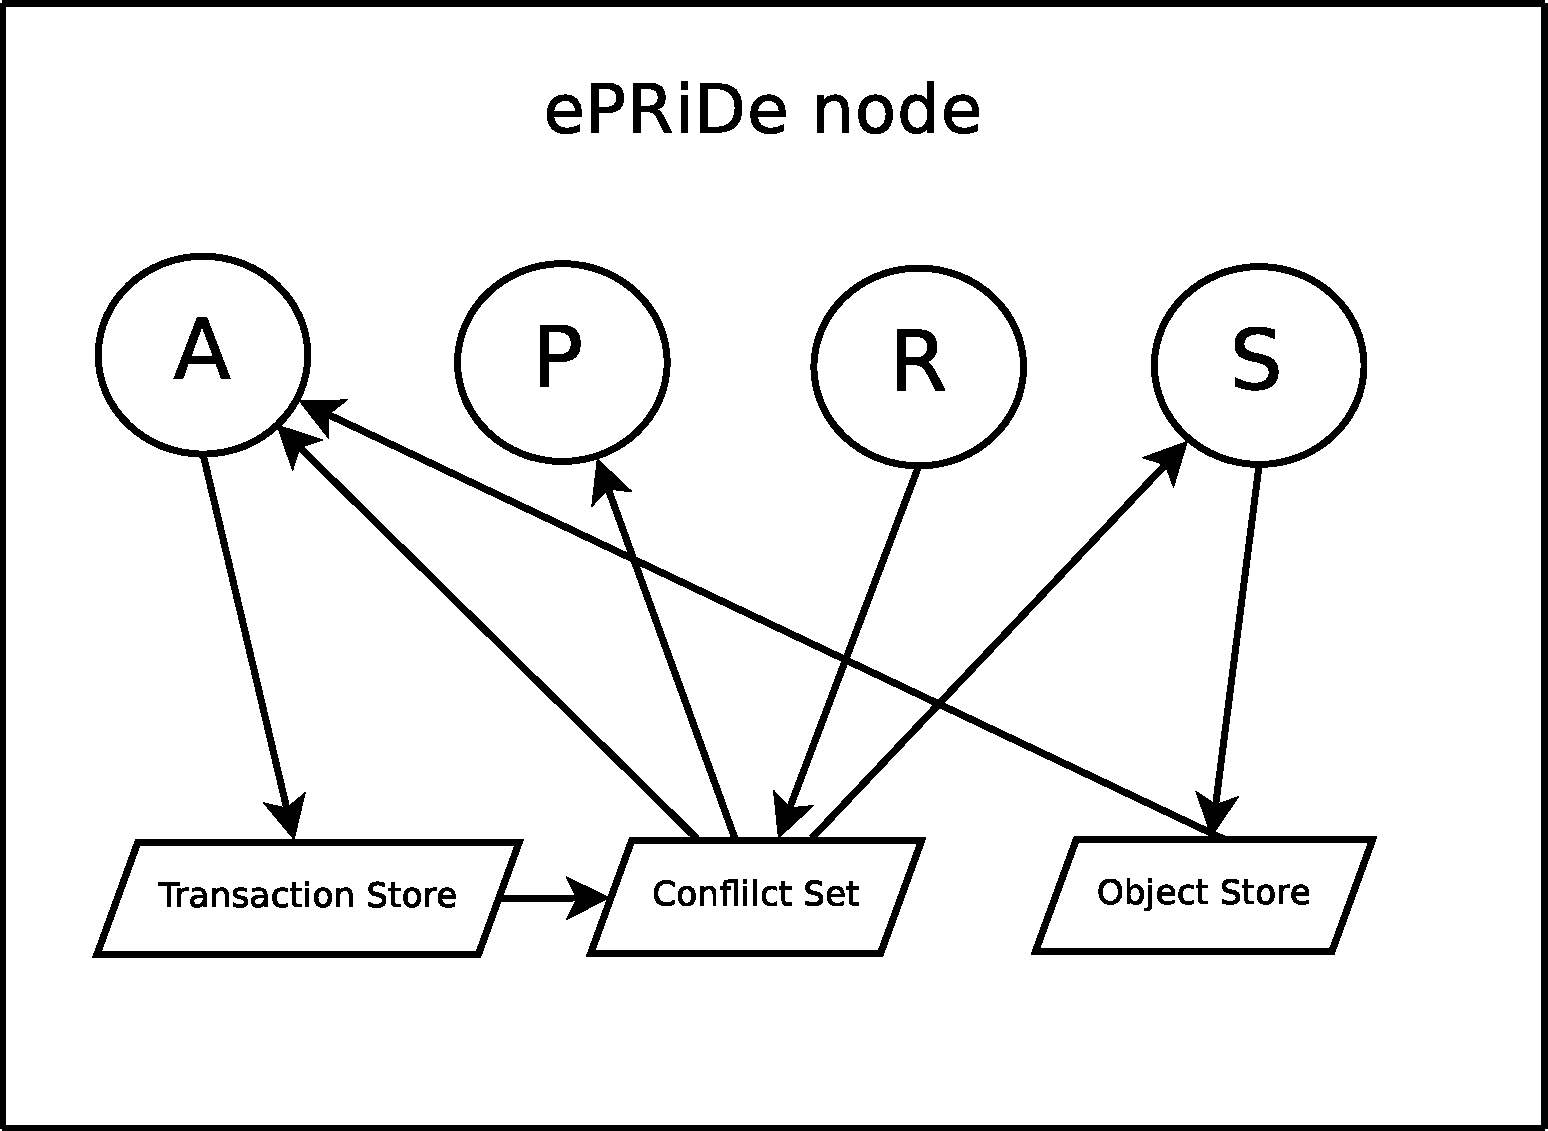
\includegraphics[height=8cm]{components.pdf}}
\caption{The components used in EPRiDe and their interactions}\label{fig:components}
\end{figure}

When an application process want to read a stable object, the read routine fetches the object state from the object store. If the application process wants to read a optimistic object, the following tasks are performed: 
\begin{enumerate}
	\item A stable version of the object are fetched from the object store.
	\item If there are any generations in the conflict set for the given object, these are resolved by the Stabilizater. The Stabilizater stabilizates each generation by perfoming a conflict resolution routine on each generation. 
	\item Each generation that is stabilized, the outcome of the conflict resolution are performed on the object. 
	\item The read process returns the optimistic object after each unstable update have been performed.
\end{enumerate}


% subsection data_interaction (end)

%(fold)

%Each EPRiDe instance contains a number of components:
% 	- Application 
% 		This component is responsible for handling read and write requests that an application can make. This includes transaction commands. 
%
%	- Propagater
%		The propagater is responsible for sending updates that are in the conflict set to the other EPRiDe instances. The propagater is used  when a commit has been performed on the node and the informmation needs to be replicated to the other EPRiDe instances.

%	- Receiver 
%		This component receives propagation messages that are send from other EPRiDe nodes. The receiver receives each message, unpacks the message and puts the information into the correct generation.

%	- Stabilizater 
%		This component performs stabilization on each generation when needed. 

% To be able to serve these components, a number of datastructures are used. A transaction store are used by the application to store transaction informantion. This information contains the operations that have been conducted inside the transaction and the object state with each operation. This is similar to a write-ahead log [ref here]. A conflict set is used to handle the different generation on a specific object. 

% - Describe replication 
% - Describe each module
% 	- Why, when 
%		- Application 
%		- Receiver 
%		- Propagater
%		- Stabilizator
%	
% - Describe the flow in number of activity diagrams
% (end)

\newpage
%!TEX root = /Users/high/Documents/School/Thesis/report/thesis.tex
\section{The Experiments} % (fold)
\label{sec:experiments}

This section explains the experiments that have been performed to measure the performance with EPRiDe and BDBe. The performance metrics that are used are detailed in the section below.
% section the_experiments (end)

\subsection{Performance metrics} % (fold)
\label{sub:experiments_performance_metrics}

To be able to measure the performance in the EPRiDe implementation a number of performance metrics have been established. These performance metrics are measured both against EPRiDe and Berkeley DB which has been extended with distributed-master replication. This extension will be referred as Berkeley DB extended (BDBe). These performance metrics have been selected due to the fact that they can be measured in single-master replication and in multi-master replication.

\begin{description}

	\item[Bandwidth usage]

This metric is measured can be measured in two ways. Measuring the amount of data traffic that gets transfered between two database nodes in the network or measuring the total number of data that is transfered between all the replicas in the network during the entire experiment.

	\item[Execution time]

	This metric measures the time it takes to process all transactions and to the time when all replicas has the same information about all objects that have been updated. For PRiDe, this means that the time for receive all transactions, perform local integration, propagate to all the replicas, perform integration on the target replica, and finally perform stabilization on target replica. For DDB, it is the time for receiving all transactions, and performing a distributed transaction update each replica. For BDBe, it is to process all transactions and for each transaction, perform local integration on the master node, and then replicate the update to the slave replicas and perform integration on the each slave. When only one node receives the updates. If all nodes can receive updates, execution time for BDBe is the time to receive all transactions, send all transactions to the master node, propagate the updates to the replicas and then integrate the update on the target replica.

	%This is the time it takes for each database node to process each transaction and perform a commit or abort on the transaction, and then replicate the update to the other database nodes and integrate the update and the database node. 

	\item[Stabilization time]
	This mean the time from that a update has reached a replica and until the update is stable on that replica. This is only measurable on PRiDe because there is no stabilization in DDB, and in BDBe, the stabilization time is from the time when the local integration has performed on master nod and until the update has been propagated to the target replicas and have been integrated on target replicas. But these is not stabilization, it is just replication of an update.

	In PRiDe, this can be measured on individual node, by measuring the time it take from that an update has been locally integrated on the replica and to the time when the update have been moved to the stable prefix. This includes the time it takes to perform conflict resolution. 

	The type of measurements can be compared between different replicas. This means that measurements can done by the maximum time, minimum time, average time, when comparing with all replicas in the network. 

	%This is the time it take for each database to process each transaction, commit or abort locally and then replicate the update to the remove database nodes, and integrate the update, and finally pertform stabilization on the updates so that all database replicas have the same information about all objects.

	\item[Blocking time] 

	When only one node (master node) is allowed to perform updates, the blocking time for PRiDe is only the time it takes to make a integration of the update on the local node. For DDB, the blocking time is the time when the transaction waits until all (or some) of the replicas has integrated the update. For BDBe, this means that blocking time will just be the local blocking time for performing the commit.
	When independent updates are allowed, it is the same blocking time for PRiDe, but for BDBe, each transaction need to wait for the transaction to be send to the master node and integrate the update on the master and then receive a reply. The blocking time for BDBe can be affected by network latency and network partitioning. For DDB, independent updates can't be used since only one node (master node) can receive updates.

\end{description}

% subsection performance_metrics (end)

%\subsection{Requirements on platform} % (fold)
%\label{sub:s}

%In order to create an implementation of PRiDe, there is a number of requirements that needs to be fulfilled to be able to perform a correct implementation.

% Main-memory storage
% Eventual Consistency 
% Optimistic replication
% Multi-master updates (Independent updates)

% subsection s (end)

% section section_name (end)

\newpage

\section{Implementation} % (fold)
\label{sec:implementation}

% section implementation (end)	


% section performance_metrics (end)

\subsection{Requirements on platform} % (fold)
\label{sub:s}

%In order to create an implementation of PRiDe, there is a number of requirements that needs to be fulfilled to be able to perform a correct implementation.

% Main-memory storage
% Eventual Consistency 
% Optimistic replication
% Multi-master updates (Independent updates)

% subsection s (end)

% section section_name (end)

\section{The experiments} % (fold)
\label{sec:the_experiments}

This section explains the different experiments that where conducted to perform the evaluation. 

\section{Results} % (fold)
\label{sec:results}

In this section, the results from the experiments that where performed are described. 

% section  (end)
\section{Related work} % (fold)
\label{sec:future_work}

This section describes other work that have been performed in optimistic replication with forward conflict resolution.

% section future_work (end)
\section{Conclusions} % (fold)
\label{sec:conclusion}

% (end)

\subsection{Performance evaluation} % (fold)
\label{sub:performance_evaluation}

In this section, conclusions are presented that are based on the experiments that have been conducted and the performance metrics.

\subsection{Future work} % (fold)
\label{sub:future_work}

(((( Add discussion about fault tolerance and diskless recovery ))))

\newpage

\bibliographystyle{agsm}
\addcontentsline{toc}{section}{Referenses}
\bibliography{thesis}

\end{document}
